% \begin{frame}{Resultados}
%   \begin{itemize}
%     \item Precipitação de carbonetos foi observada por Toji, Miyamoto and Raabe\footnotemark[1] e Nayak et al\footnotemark[2] durante T\&P de aços de médio e alto carbono
%     \item Toji: PT = 400°C/5 min; aço era altamente ligado em manganês, o que justifica a ausência de produtos bainíticos
%   \end{itemize}

%   \begin{figure}
%     \centering
%     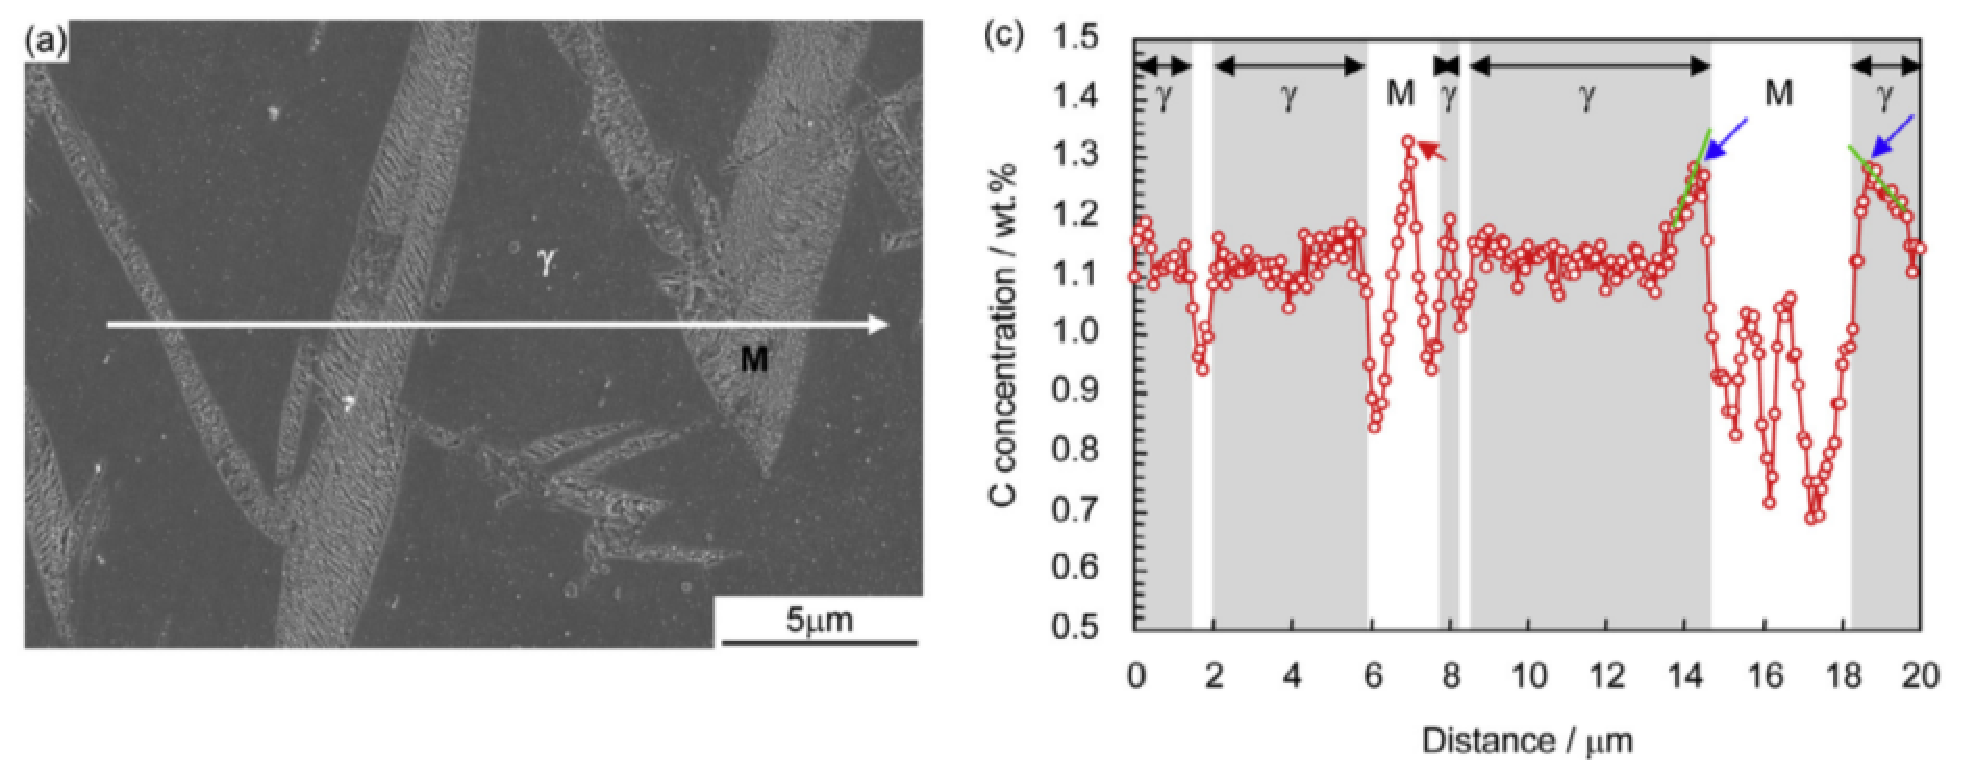
\includegraphics[width=\textwidth]{img/toji_2015.pdf}
%   \end{figure}

%   \footnotetext[1]{Toji Y, Miyamoto G, Raabe D. Acta Mater 2015; vol 86, pp 137}
%   \footnotetext[2]{Nayak SS et al. Materials Science and Engineering A 2008; vol 498, pp 442-456}
% \end{frame}

% \begin{frame}{Resultados}
%   \begin{itemize}
%     \item Nayak: Carbonetos $\varepsilon$ durante T\&P em temperaturas tão baixas quanto 250 °C (1.7\%Si e 1,5\%Cr) 
%     \item Possível ocorrência de reação bainítica não é discutida, provavelmente devido alto teor de Cr.
%   \end{itemize}

%   \begin{figure}
%     \centering
%     \includegraphics[width=.8\textwidth]{img/nayak2008.pdf}
%   \end{figure}
% \end{frame}

% \begin{frame}{Resultados}
%   \begin{itemize}
%     \item Carbonetos não poderiam ser vistos em temperaturas de partição mais baixas...?
%     \item Têmpera subzero ($N_2$ líquido) + revenimento contínuo (até 700 °C a 0,2 °C/s) no dilatômetro Bähr e na XTMS
%     \item Informações: dilatação, largura e \textit{d} do pico $(110)\alpha$
%   \end{itemize}

%   \begin{figure}
%     \centering
%     \includegraphics<1>[width=.8\textwidth]{img/XTMS/FoFo-subzero_tempering-continous_2.eps}
%     \includegraphics<2>[width=.8\textwidth]{img/XTMS/FoFo-subzero_tempering-continous_1.eps}
%     \includegraphics<3>[width=.8\textwidth]{img/XTMS/FoFo-subzero_tempering-continous_1-comments.pdf}
%   \end{figure}
% \end{frame}


% \begin{frame}{Resultados}
%   \begin{itemize}
%     \item DRX na linha XTMS usando detector 2D. Tempo de exposição: 1 minuto
%     \item Grande amostragem (anéis de difração): sinal/ruído $\uparrow$
%   \end{itemize}

%   \begin{figure}
%     \centering
%     \includegraphics<1>[width=\textwidth]{img/XTMS/FoFo-QP_Rayonix.eps}
%     \includegraphics<2>[width=\textwidth]{img/XTMS/FoFo-QP_Rayonix_markers.pdf}
%   \end{figure}
% \end{frame}


% \begin{frame}{Resultados}
%   \begin{itemize}
%     \item Picos alargados justificariam precipitados muito finos (equação de Scherrer)
%   \end{itemize}

%   \begin{figure}
%     \centering
%     \includegraphics[width=\textwidth]{img/XTMS/FoFo-QP_Rayonix_zoom.eps}
%   \end{figure}
% \end{frame}
